\section{Generalization: Why Fitting the Data Is Not Enough}

The previous sections introduced the population objective of learning and the ideal benchmark given by Bayes-optimal prediction. We now encounter the central difficulty of the subject: the learner does not observe the population distribution directly. It sees only a finite sample. The real question is therefore not whether a model can fit the observed data, but whether it can use those data to perform well on new examples drawn from the same environment.

This distinction between fitting and future performance is the conceptual core of generalization theory.

\subsection*{Training error, test error, and the generalization gap}

Let
\[
\mathcal D=\{(X_i,Y_i)\}_{i=1}^n
\]
be a training sample, let $f$ be a predictor, and let $\ell$ be a loss function.

\begin{definition}[Training error]
The \emph{training error} or \emph{training risk} of $f$ on $\mathcal D$ is its empirical risk on the sample used for fitting:
\[
\widehat R_n(f)=\frac1n\sum_{i=1}^n \ell(f(X_i),Y_i).
\]
\end{definition}

\begin{definition}[Test error]
The \emph{test error} of $f$ is its performance on fresh data not used in training. At the population level, this is measured by the expected risk
\[
R(f)=\mathbb E[\ell(f(X),Y)].
\]
If one has an independent test sample
\[
\mathcal D_{\mathrm{test}}=\{(X_i',Y_i')\}_{i=1}^m,
\]
then the corresponding empirical test error is
\[
\widehat R_{\mathrm{test}}(f)=\frac1m\sum_{i=1}^m \ell(f(X_i'),Y_i').
\]
\end{definition}

\begin{definition}[Generalization gap]
The \emph{generalization gap} of $f$ is the difference between population risk and training risk:
\[
\mathrm{Gen}(f)=R(f)-\widehat R_n(f).
\]
\end{definition}

A model generalizes well when two things happen at once:

\begin{enumerate}
    \item its training error is a reliable guide to its test error, so the generalization gap is small;
    \item its test error itself is small.
\end{enumerate}

These are different requirements. A model may have a tiny generalization gap but still perform badly if both training and test error are large. Conversely, it may have tiny training error and still perform badly if the generalization gap is large.

\subsection*{Why fitting the training sample is not enough}

The following proposition states the basic warning formally.

\begin{proposition}[Minimizing training error alone does not guarantee low test error]
There exist learning problems and hypothesis classes for which a predictor achieves zero training error while having arbitrarily poor population performance.
\end{proposition}

\begin{proof}
Take any finite training sample
\[
\mathcal D=\{(x_1,y_1),\dots,(x_n,y_n)\}.
\]
Consider a hypothesis class rich enough to contain all functions from $\mathcal X$ to $\mathcal Y$. Then there exists a predictor $f_{\mathrm{mem}}$ such that
\[
f_{\mathrm{mem}}(x_i)=y_i
\qquad\text{for all } i=1,\dots,n,
\]
while the values of $f_{\mathrm{mem}}(x)$ for inputs outside the training sample are assigned arbitrarily.

By construction,
\[
\widehat R_n(f_{\mathrm{mem}})=0
\]
under zero--one loss. However, because the outputs away from the observed points are unconstrained, the expected risk $R(f_{\mathrm{mem}})$ can be large. Thus perfect training performance does not imply good performance on future data.
\end{proof}

The proposition is simple, but its message is profound. Learning cannot be identified with memorization. A predictor that merely reproduces the sample may look successful from the viewpoint of training error while failing completely at the actual task of prediction beyond the sample.

\begin{figure}[tbp]
\centering
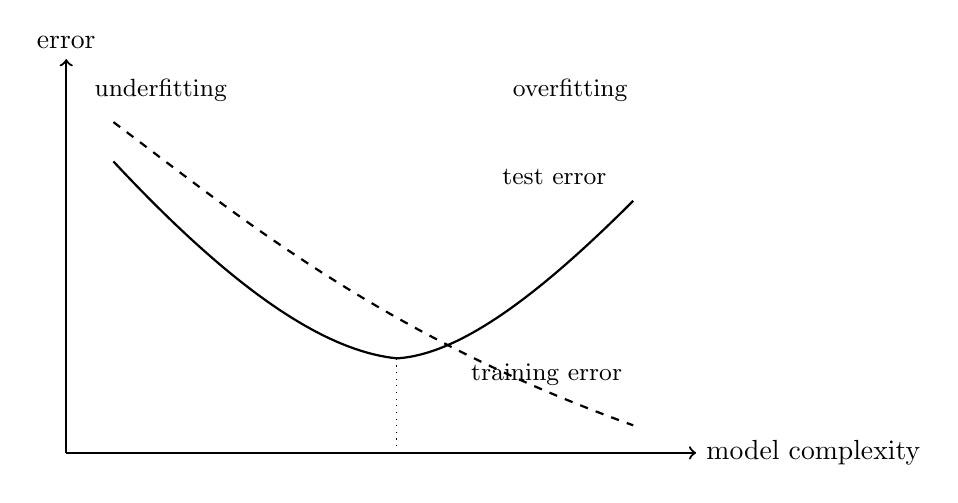
\begin{tikzpicture}[scale=1, every node/.style={align=center}]
    \draw[->, thick] (0,0) -- (8,0) node[right] {model complexity};
    \draw[->, thick] (0,0) -- (0,5) node[above] {error};

    % training error curve
    \draw[thick, dashed]
        (0.6,4.2) .. controls (2.2,3.0) and (4.0,1.5) .. (7.2,0.35);
    \node at (6.1,1.0) {\small training error};

    % test error curve
    \draw[thick]
        (0.6,3.7) .. controls (2.0,2.2) and (3.2,1.3) .. (4.2,1.2)
        .. controls (5.0,1.25) and (6.0,2.0) .. (7.2,3.2);
    \node at (6.2,3.5) {\small test error};

    \draw[dotted] (4.2,0) -- (4.2,1.2);
    \node at (1.2,4.6) {\small underfitting};
    \node at (6.4,4.6) {\small overfitting};
\end{tikzpicture}
\caption{A schematic picture of underfitting and overfitting. As model complexity increases, training error usually decreases, but test error may first decrease and then rise if the model begins to fit sample-specific noise rather than stable structure.}
\end{figure}

\subsection*{Underfitting and overfitting}

Two characteristic failures organize much of the intuition of generalization.

\paragraph{Underfitting.}
A model may be too rigid to capture the relevant structure in the data. Then it performs poorly even on the training sample and also poorly on new data. This is \emph{underfitting}.

\paragraph{Overfitting.}
A model may be so flexible that it adapts not only to signal but also to accidental idiosyncrasies of the sample. Then it may achieve very low training error while suffering noticeably worse test error. This is \emph{overfitting}.

These are not merely verbal opposites. They reflect two distinct ways in which learning can fail:

\begin{itemize}
    \item the model class may be too simple to represent the target structure;
    \item the model class may be so rich that finite data do not constrain it reliably.
\end{itemize}

\subsection*{Model complexity and sample size}

Generalization depends on a balance between the expressive power of the hypothesis class and the amount of information supplied by the data.

A richer hypothesis class can represent more patterns, but it can also fit more accidental fluctuations. A larger sample gives stronger evidence about which patterns are stable and which are merely noise. This leads to a basic qualitative principle:

\begin{quote}
Complex models generally require more data to generalize reliably.
\end{quote}

This principle is only qualitative at present. Later chapters will make it precise using capacity measures and probability bounds. But even before that theory is introduced, the core idea is already visible: \emph{model complexity and sample size must be matched}.

\begin{figure}[tbp]
\centering
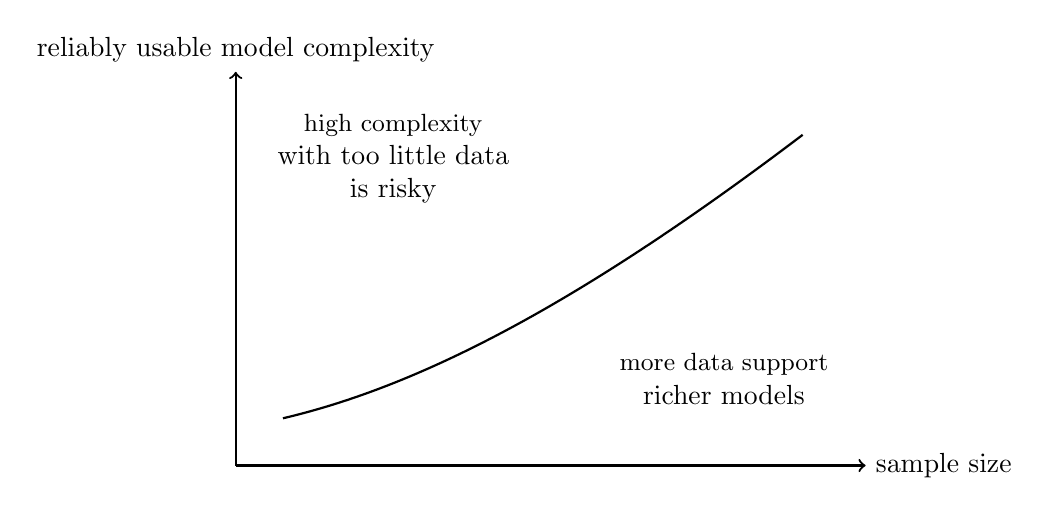
\begin{tikzpicture}[scale=1, every node/.style={align=center}]
    \draw[->, thick] (0,0) -- (8,0) node[right] {sample size};
    \draw[->, thick] (0,0) -- (0,5) node[above] {reliably usable model complexity};

    \draw[thick] (0.6,0.6) .. controls (2.3,1.0) and (4.3,2.0) .. (7.2,4.2);

    \node at (2.0,3.9) {\small high complexity\\with too little data\\is risky};
    \node at (6.2,1.1) {\small more data support\\richer models};
\end{tikzpicture}
\caption{A schematic relation between sample size and usable model complexity. As more data become available, richer hypothesis classes can often be estimated more reliably.}
\end{figure}

\subsection*{A uniform-convergence intuition}

The previous section showed that empirical risk is unbiased for a fixed predictor. But learning does not select a predictor in advance. It chooses one \emph{after seeing the data}. This is why the fixed-function argument is not enough.

A natural stronger requirement is that empirical risk should approximate population risk \emph{uniformly} over the whole hypothesis class:
\[
\sup_{f\in\mathcal H}\big|R(f)-\widehat R_n(f)\big|.
\]
If this quantity is small, then no predictor in the class can look much better on the training sample than it truly is on the population. In that regime, minimizing empirical risk is sensible because training performance is uniformly trustworthy across the class.

At a conceptual level, this is one of the first explanations of why generalization can happen:
the sample is large enough, relative to the complexity of the hypothesis class, that empirical comparisons reflect genuine population comparisons.

\subsection*{A high-level decomposition of excess risk}

Section 1.2 already introduced the approximation/estimation/optimization trichotomy. It is worth repeating it here because it explains why generalization is not a one-dimensional problem.

\begin{proposition}[A high-level decomposition of excess risk]
Let $f^\star$ denote the Bayes-optimal predictor, let
\[
f_{\mathcal H}^\star \in \arg\min_{f\in\mathcal H} R(f)
\]
be the best predictor in the chosen hypothesis class, let
\[
f_n^\star \in \arg\min_{f\in\mathcal H} \widehat R_n(f)
\]
be an empirical risk minimizer in the class, and let $\hat f_n$ be the predictor actually returned by the learning algorithm. Then
\[
R(\hat f_n)-R(f^\star)
=
\underbrace{\bigl(R(f_{\mathcal H}^\star)-R(f^\star)\bigr)}_{\text{approximation}}
+
\underbrace{\bigl(R(f_n^\star)-R(f_{\mathcal H}^\star)\bigr)}_{\text{estimation}}
+
\underbrace{\bigl(R(\hat f_n)-R(f_n^\star)\bigr)}_{\text{optimization}}.
\]
\end{proposition}

\begin{proof}
Add and subtract $R(f_{\mathcal H}^\star)$ and $R(f_n^\star)$:
\[
R(\hat f_n)-R(f^\star)
=
\bigl(R(\hat f_n)-R(f_n^\star)\bigr)
+
\bigl(R(f_n^\star)-R(f_{\mathcal H}^\star)\bigr)
+
\bigl(R(f_{\mathcal H}^\star)-R(f^\star)\bigr).
\]
This is exactly the stated decomposition.
\end{proof}

This decomposition is useful because it separates three sources of difficulty:

\begin{itemize}
    \item \textbf{Approximation error:} the class $\mathcal H$ may be too limited to represent the ideal predictor well.
    \item \textbf{Estimation error:} finite data may not identify a nearly optimal member of $\mathcal H$ reliably.
    \item \textbf{Optimization error:} the training procedure may fail to find the empirical minimizer.
\end{itemize}

So when a learner performs badly, the reason may be expressive limitation, finite-sample uncertainty, or optimization failure. Generalization sits mainly in the second term, but practical learning depends on all three.

\subsection*{Bias and variance}

A classical way to think about generalization is through the distinction between \emph{bias} and \emph{variance}.

\paragraph{Bias.}
Bias reflects systematic error caused by a restrictive model class or learning rule. A high-bias method tends to miss important structure even if given more data.

\paragraph{Variance.}
Variance reflects instability with respect to the training sample. A high-variance method may produce very different predictors when trained on different datasets drawn from the same population.

At a fixed input $x$, if $\hat f(x)$ is the prediction produced by a random training sample and $f^\star(x)$ is the target benchmark, then one common schematic decomposition is
\[
\mathbb E\big[(\hat f(x)-f^\star(x))^2\big]
=
\big(\mathbb E[\hat f(x)]-f^\star(x)\big)^2
+
\mathbb E\Big[\big(\hat f(x)-\mathbb E[\hat f(x)]\big)^2\Big].
\]
The first term is the squared bias and the second is the variance.

\begin{figure}[tbp]
\centering
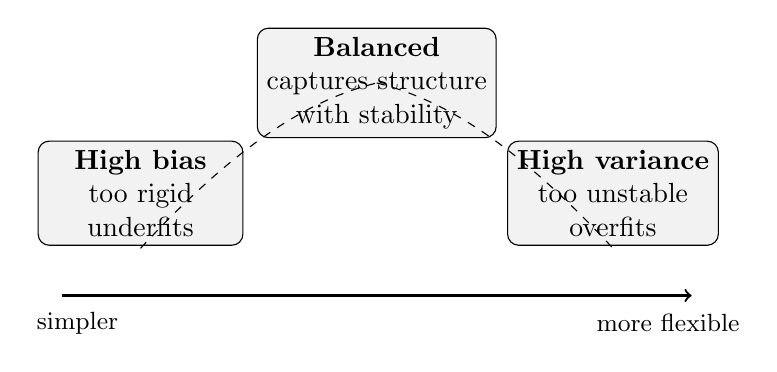
\begin{tikzpicture}[scale=1, every node/.style={align=center}]
    \node[draw, rounded corners, fill=gray!10, minimum width=2.6cm, minimum height=1cm] (bias) at (2,1.8) {\textbf{High bias}\\too rigid\\underfits};
    \node[draw, rounded corners, fill=gray!10, minimum width=2.6cm, minimum height=1cm] (balance) at (5,3.2) {\textbf{Balanced}\\captures structure\\with stability};
    \node[draw, rounded corners, fill=gray!10, minimum width=2.6cm, minimum height=1cm] (var) at (8,1.8) {\textbf{High variance}\\too unstable\\overfits};

    \draw[->, thick] (1.0,0.5) -- (9.0,0.5);
    \node at (1.2,0.15) {\small simpler};
    \node at (8.7,0.15) {\small more flexible};

    \draw[dashed] (2,1.1) .. controls (3.3,2.5) and (4.2,3.0) .. (5,3.2);
    \draw[dashed] (5,3.2) .. controls (5.8,3.0) and (6.7,2.5) .. (8,1.1);
\end{tikzpicture}
\caption{A schematic bias--variance picture. Simpler models tend to have higher bias and lower variance; more flexible models tend to have lower bias and higher variance. Good generalization usually requires a balance between the two.}
\end{figure}

The bias--variance language is especially useful in introductory regression settings. It is not a complete explanation of all modern deep-learning behavior, but it remains a valuable first lens on the tradeoff between expressiveness and stability.

\subsection*{Regularization and cross-validation at a conceptual level}

Two practical responses to overfitting appear early in almost every area of machine learning.

\paragraph{Regularization.}
Instead of minimizing empirical risk alone, one may penalize complexity:
\[
\min_{f\in\mathcal H} \widehat R_n(f)+\lambda\,\Omega(f),
\]
where $\Omega(f)$ measures some notion of complexity and $\lambda>0$ controls the strength of the penalty. The goal is not merely to fit the sample, but to favor predictors that are stable enough to perform well beyond it.

\paragraph{Cross-validation.}
Because the true population risk is unknown, one often estimates predictive performance by separating fitting from evaluation. Conceptually, cross-validation proceeds by splitting the available data into parts, training on one part, evaluating on another, and repeating this process across several splits. Its role is to imitate the train/test distinction using only the available sample.

Cross-validation does not replace theory, but it encodes a crucial practical lesson: evaluation on the same data used for fitting can be misleading.

\commonconfusion{Overfitting is not the same thing as ``having many parameters'' in every regime. A large model can overfit, but whether it does so depends on the data, the optimization procedure, the inductive bias of the architecture, the amount of regularization, and the structure of the task. Parameter count alone is too crude to explain generalization.}

\whattoremember{Generalization is the ability to perform well on new data, not merely on the training sample. Training error, test error, and the generalization gap are different quantities. Minimizing training error alone does not guarantee low test error. Good generalization depends on the interaction among model complexity, sample size, inductive bias, and optimization. A useful high-level guide is the decomposition of excess risk into approximation, estimation, and optimization terms, while the classical bias--variance picture provides an intuitive first explanation of underfitting and overfitting.}

\subsection*{Exercises}

\begin{exercise}
Define in your own words the difference between training error, test error, and the generalization gap. Why can a model have small training error but large test error?
\end{exercise}

\begin{exercise}
Construct a simple example of a predictor that memorizes a finite training set. Explain why zero training error does not certify learning in the predictive sense.
\end{exercise}

\begin{exercise}
Suppose two model classes are available for the same task: one very simple and one highly flexible. Describe a situation in which the simple model underfits and a situation in which the flexible model overfits.
\end{exercise}

\begin{exercise}
Cross-validation is often used to choose hyperparameters such as model complexity or regularization strength. Explain conceptually why evaluating all candidate models only on the training set is unreliable, and how cross-validation attempts to correct this.
\end{exercise}

\begin{exercise}
In the decomposition
\[
R(\hat f_n)-R(f^\star)
=
\text{approximation}+\text{estimation}+\text{optimization},
\]
describe one concrete reason each term might be large in practice.
\end{exercise}

\begin{exercise}
Why is it misleading to define overfitting simply as ``using too many parameters''? Give at least two other factors that influence whether a model generalizes well.
\end{exercise}

\subsection*{Notes and references}

This section introduces the central distinction between fitting the observed sample and performing well on future data. The language of training error, test error, and generalization gap is foundational for the rest of learning theory. The underfitting/overfitting picture, the qualitative relation between model complexity and sample size, the approximation/estimation/optimization decomposition, and the bias--variance viewpoint are all first-pass frameworks rather than final explanations. Later chapters will revisit these ideas with more precise tools, including capacity measures, concentration arguments, regularization theory, and modern perspectives on overparameterized learning.